\chapter{Object-oriented programming}
\label{chap:oop}

\idx{Object-oriented programming} is a programming paradigm that focusses on \idx{objects} such as a person, place, thing, event, and concept relevant for the problem. Objects may contain data and code, which in the object-oriented paradigm are called \idx{attributeds} and \idx{methods}. Object-oriented programming is an extension of data types, in the sense that objects contains both data and functions in a similar manner as a module, but object-oriented programming emphasizes the semantic unity of the data and functions. Thus, objects are \idx{models} of real world entities, and object-oriented programming leads to a particular style of programming analysis and design called \idx[object-oriented analysis]{object-oriented analysis and design}\idxs{object-oriented design}. 

Before we dive into the details of the language support for object-oriented programming ing F\#, we will first introduce central elements of object-oriented analysis and design. The analysis serves as input to the design phase, where the analysis reveals \idx{what} a program is supposed to do, and the design \idx{how} it is supposed to be doing i. The analysis should be expressed in general terms irrespective of the technologic constraints, while the design should include technological constraints such as defined by the targeted language and hardware. 

\section{Object-oriented Analysis}
The primary task of \idx{object-oriented analysis} is to 
\begin{itemize}
\item identify objects,
\item describe object behaviour,
\item describe object interactions, and 
\item describe some details of the object's inner workings.
\end{itemize}
We will now illustrate, how an object-oriented analysis could be performed by applying the above tasks to the for the above problem. Consider the following \idx{problem statement}:
%
\begin{problem}
  Write a racing game, where each player controls his or her vehicle on a set track. Each vehicle must have individual features such as top acceleration, speed, and handling. The player must be able to turn the vehicle left and right, and to accelerate up and down. At the beginning of the game, each vehicle is placed behind the starting line. Once the start signal is given, then the players may start to operate their vehicles. The player who first completes 3 rounds wins.
\end{problem}
%
\textbf{Identification of objects:} To identify objects we seek relevant persons, places, things, events, concept etc., which are almost always characterized by being \idx{nouns} in the text. E.g., in the above the following nouns seems relevant: 
\begin{quote}
  game, player, vehicle, track, feature, starting line, start signal
\end{quote}
In the object-oriented paradigm, the objects has a type, which is called a \idx{class}, and each value or variable of a particular class is called and \idx{instance} of a class or simply just and \idx{object}. Many languages include F\# include support for \idx{static} attributes and methods, which essentially implies that the class reverts to becoming a name spaces or a module, but we will ignore for the moment. 

A key point in object-oriented programming is that objects should to a large extend be independent and reusable. As an example the type \lstinline|int| models the concept of integer numbers. It can hold integer values from -2,147,483,648 to 2,147,483,647, and a number of standard operations and functions are defined for it. We may use integers in many different programs, and it is certain that the original designers did not foresee our use, but strived to make a general type applicable for many uses. Such a design is a useful goal, when designing objects, that is, our objects should model the general concepts and be applicable in future uses.

\textbf{Object behaviour and interactions:} We are still far from having a program design, that we can implement in F\#. To continue our object-oriented design, Let's consider some of the object candiate identified above, and verbalize how they would act as models of general concepts useful in our game.
\begin{description}
\item[player] A player interacts with the game and could be a human or computer player. A player must in general be able to control the vehicle and receive information about the track and all vehicles or at least some information about the nearby vehicles and track. And the player must receive information about the state of the game, i.e., when does the race start and stop.
\item[vehicle] A vehicle is a model of a physical object, which moves around on the track under the influence of a player. A vehicle must have a number of attributes such as top acceleration, speed, and handling, and must be able to receive information about when to turn and accelerate. A vehicle must be able to determine its location in particular if it is on or off track and, and it must be able to determine if it has crashed into an obstacle such as another vehicle.
\item[track] A track is a fixed entity on which they vehicles race. It has a size and a shape, a starting and a finishing line, which may be the same, and vehicles are placeable on the track and can move on and possibly off the track.
\end{description}
From the above we see that the object candidates 'feature' seems to be a natural part of the description of the vehicle's attributes, and similarly, 'starting line' may be an intricate part of a track. Also, many of the \idx{verbs} used in the problem statement and in our extended verbalisation of the general concepts indicate methods that are used to interact with the object. Here it is important to maintain an object centered perspective, i.e., for a general purpose vehicle object, we need not include information about the player, analogous to a value of type \lstinline|int| need not know anything the program, in which it is being used. In contrast, the candidate 'game' is not as easily dismissed and could be used as a class which contains all the above, i.e.,
\begin{description}
\item[game] A game is the total sum of all the players, the vehicles, the tracks, and their interactions. A game controls the flow of a particular game including inviting players to race, sending the start signal, and monitoring when a game is finished and who won.
\end{description}
With this description we see that 'start signal' can be included as a natural part of the game object. Being confident that a good working hypothesis of the essential objects for the solution, we continue our investigating into further details about the objects and their interactions.

\textbf{Analysis details:} To describe the objects and their interaction we will use a \idx{class diagram}. A class diagram is a schematic drawing of the program highlighting its object-oriented structure and we will use the \idx{Universal Modelling Language 2} (\idx{UML}) \cite{uml2} standard. A class is drawn as a 

\begin{figure}
  \centering
  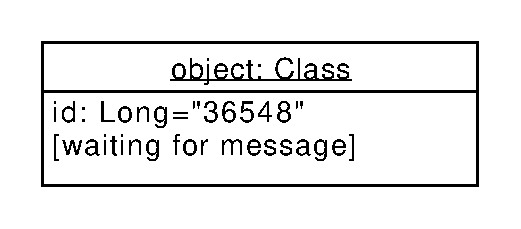
\includegraphics[width=0.3\linewidth]{carRace}
  \caption{An example of UML, produced by using UMLet \cite{umlet}}
  \label{uml}
\end{figure}

Things to remember: 
\begin{itemize}
\item upcast and downcast \keyword{upcast}, \lexeme{:>},
  \keyword{downcast}, \lexeme{:?>}
\item boxing \lstinline|(box 5) :?> int;;|, see Spec-4.0 chapter
  18.2.6.
\item obj type Spec-4.0 chapter 18.1
\item boxing Spec-4.0 Section 18.2.6
\end{itemize}

\jon{In object oriented programming: functions and data are
  combined. Contrast the Anemic Domain Model (\url{https://www.martinfowler.com/bliki/AnemicDomainModel.html})}
%%% Local Variables:
%%% TeX-master: "fsharpNotes"
%%% End:
